\documentclass[11pt,a4paper]{article}
\usepackage[margin=2.2cm]{geometry}
\usepackage{graphicx}
\usepackage{booktabs}
\usepackage{array}
\usepackage{longtable}
\usepackage{threeparttable}
\usepackage{pdflscape}
\usepackage{caption}
\usepackage{float}
\usepackage{xcolor}
\usepackage{xurl}
\usepackage[colorlinks=true,linkcolor=blue!55!black,urlcolor=blue!55!black]{hyperref}
\usepackage{microtype}
\graphicspath{{../figures/supplementary/}}
\setlength{\parindent}{0pt}
\setlength{\parskip}{5pt}
\setlength{\emergencystretch}{3em}
\captionsetup{font=small,labelfont=bf}
\renewcommand{\tablename}{Supplementary Table}
\renewcommand{\thetable}{S\arabic{table}}
\renewcommand{\figurename}{Supplementary Figure}
\renewcommand{\thefigure}{S\arabic{figure}}

\begin{document}

\begin{center}
{\Large\bfseries Supplementary Information\par}
\vspace{8pt}
{\large An Accuracy and Calibration Benchmark of scGPT Pipelines and Matched Classical Models for Cell Type Annotation\par}
\vspace{8pt}
Alireza Khosravi et al.
\end{center}

\section*{Contents and scope}

This document reports the complete numerical outputs underlying the revised manuscript. It includes all 36 within-atlas pipelines, paired differences, every donor-fold result, donor- and cell-bootstrap comparisons, all label-scarcity settings, temperature-scaling results, computational identifiers, and reliability diagrams with bin counts and uncertainty. Results derived from the superseded custom wrapper, end-to-end fine-tuning, or embedding-based gene-similarity analysis are not included.

\begin{itemize}
\item Supplementary Table S1: all within-atlas discrimination and calibration metrics.
\item Supplementary Table S2: paired within-atlas Macro F1 differences.
\item Supplementary Table S3: all five donor-held-out folds and six pipelines.
\item Supplementary Table S4: donor versus cell uncertainty and paired donor differences.
\item Supplementary Table S5: complete label-scarcity results.
\item Supplementary Table S6: complete temperature-scaling results.
\item Supplementary Tables S7--S8: dataset, checkpoint, and software audit.
\item Supplementary Figures S1--S6: within-atlas reliability diagrams.
\item Supplementary Figure S7: donor-held-out reliability diagrams.
\end{itemize}

\begin{landscape}
\scriptsize
\setlength{\tabcolsep}{2.6pt}
\begin{longtable}{llccccccccc}
\caption{Complete within-atlas results for all 36 representation--classifier pipelines.}\label{tab:s1}\\
\toprule Dataset & Pipeline & Macro F1 & 95\% CI & Accuracy & Bal. acc. & ECE & Adapt. & Classwise & Brier & NLL \\
\midrule\endfirsthead
\multicolumn{11}{c}{\tablename\ \thetable{} continued}\\\toprule
Dataset & Pipeline & Macro F1 & 95\% CI & Accuracy & Bal. acc. & ECE & Adapt. & Classwise & Brier & NLL \\
\midrule\endhead
\midrule\multicolumn{11}{r}{Continued on next page}\\\endfoot
\bottomrule\endlastfoot
TNBC & scGPT emb. + LR & 0.978 & 0.977--0.980 & 0.974 & 0.974 & 0.010 & 0.010 & 0.003 & 0.040 & 0.081 \\
TNBC & scGPT emb. + RF & 0.968 & 0.966--0.969 & 0.965 & 0.952 & 0.043 & 0.043 & 0.014 & 0.061 & 0.138 \\
TNBC & scGPT emb. + XGB & 0.980 & 0.979--0.981 & 0.976 & 0.975 & 0.001 & 0.002 & 0.001 & 0.036 & 0.069 \\
TNBC & Matched expr. + LR & 0.991 & 0.990--0.992 & 0.989 & 0.990 & 0.002 & 0.002 & 0.001 & 0.017 & 0.034 \\
TNBC & Matched expr. + RF & 0.987 & 0.986--0.989 & 0.986 & 0.981 & 0.032 & 0.032 & 0.010 & 0.027 & 0.067 \\
TNBC & Matched expr. + XGB & 0.992 & 0.991--0.992 & 0.990 & 0.990 & 0.002 & 0.002 & 0.001 & 0.015 & 0.030 \\
\addlinespace
Indonesia PBMC & scGPT emb. + LR & 0.929 & 0.926--0.932 & 0.924 & 0.916 & 0.021 & 0.021 & 0.004 & 0.114 & 0.210 \\
Indonesia PBMC & scGPT emb. + RF & 0.912 & 0.909--0.915 & 0.906 & 0.893 & 0.074 & 0.074 & 0.012 & 0.154 & 0.293 \\
Indonesia PBMC & scGPT emb. + XGB & 0.936 & 0.933--0.938 & 0.924 & 0.930 & 0.004 & 0.004 & 0.001 & 0.112 & 0.200 \\
Indonesia PBMC & Matched expr. + LR & 0.956 & 0.953--0.958 & 0.953 & 0.957 & 0.009 & 0.008 & 0.001 & 0.072 & 0.133 \\
Indonesia PBMC & Matched expr. + RF & 0.929 & 0.925--0.933 & 0.944 & 0.903 & 0.104 & 0.104 & 0.016 & 0.109 & 0.228 \\
Indonesia PBMC & Matched expr. + XGB & 0.955 & 0.953--0.958 & 0.952 & 0.953 & 0.004 & 0.005 & 0.001 & 0.070 & 0.124 \\
\addlinespace
Brain atlas & scGPT emb. + LR & 0.871 & 0.831--0.902 & 0.984 & 0.812 & 0.025 & 0.025 & 0.006 & 0.029 & 0.082 \\
Brain atlas & scGPT emb. + RF & 0.893 & 0.857--0.920 & 0.986 & 0.835 & 0.026 & 0.027 & 0.006 & 0.029 & 0.092 \\
Brain atlas & scGPT emb. + XGB & 0.931 & 0.904--0.953 & 0.988 & 0.895 & 0.008 & 0.008 & 0.002 & 0.021 & 0.060 \\
Brain atlas & Matched expr. + LR & 0.945 & 0.925--0.962 & 0.985 & 0.937 & 0.008 & 0.008 & 0.002 & 0.025 & 0.069 \\
Brain atlas & Matched expr. + RF & 0.831 & 0.790--0.865 & 0.984 & 0.775 & 0.030 & 0.030 & 0.007 & 0.029 & 0.084 \\
Brain atlas & Matched expr. + XGB & 0.952 & 0.929--0.970 & 0.988 & 0.924 & 0.005 & 0.005 & 0.001 & 0.019 & 0.043 \\
\addlinespace
Multi-tissue TME & scGPT emb. + LR & 0.321 & 0.318--0.325 & 0.493 & 0.306 & 0.016 & 0.017 & 0.006 & 0.667 & 1.500 \\
Multi-tissue TME & scGPT emb. + RF & 0.334 & 0.325--0.345 & 0.500 & 0.306 & 0.056 & 0.055 & 0.012 & 0.660 & 1.568 \\
Multi-tissue TME & scGPT emb. + XGB & 0.365 & 0.359--0.372 & 0.506 & 0.336 & 0.010 & 0.010 & 0.004 & 0.644 & 1.442 \\
Multi-tissue TME & Matched expr. + LR & 0.357 & 0.351--0.364 & 0.501 & 0.330 & 0.012 & 0.013 & 0.007 & 0.655 & 1.463 \\
Multi-tissue TME & Matched expr. + RF & 0.391 & 0.378--0.404 & 0.534 & 0.359 & 0.024 & 0.024 & 0.007 & 0.615 & 1.514 \\
Multi-tissue TME & Matched expr. + XGB & 0.416 & 0.404--0.430 & 0.532 & 0.379 & 0.023 & 0.023 & 0.007 & 0.614 & 1.368 \\
\addlinespace
Human pancreas & scGPT emb. + LR & 0.722 & 0.717--0.727 & 0.977 & 0.713 & 0.050 & 0.050 & 0.028 & 0.044 & 0.110 \\
Human pancreas & scGPT emb. + RF & 0.743 & 0.720--0.784 & 0.979 & 0.730 & 0.045 & 0.045 & 0.024 & 0.043 & 0.099 \\
Human pancreas & scGPT emb. + XGB & 0.874 & 0.817--0.920 & 0.989 & 0.843 & 0.005 & 0.005 & 0.003 & 0.016 & 0.035 \\
Human pancreas & Matched expr. + LR & 0.983 & 0.962--0.999 & 0.998 & 0.987 & 0.001 & 0.001 & 0.001 & 0.003 & 0.005 \\
Human pancreas & Matched expr. + RF & 0.951 & 0.912--0.979 & 0.995 & 0.919 & 0.038 & 0.038 & 0.020 & 0.015 & 0.052 \\
Human pancreas & Matched expr. + XGB & 0.982 & 0.962--0.997 & 0.997 & 0.996 & 0.001 & 0.001 & 0.001 & 0.005 & 0.009 \\
\addlinespace
Pig pancreas & scGPT emb. + LR & 0.601 & 0.583--0.619 & 0.941 & 0.545 & 0.044 & 0.044 & 0.037 & 0.088 & 0.187 \\
Pig pancreas & scGPT emb. + RF & 0.596 & 0.577--0.614 & 0.938 & 0.536 & 0.052 & 0.051 & 0.038 & 0.097 & 0.198 \\
Pig pancreas & scGPT emb. + XGB & 0.865 & 0.810--0.907 & 0.972 & 0.796 & 0.011 & 0.011 & 0.010 & 0.043 & 0.087 \\
Pig pancreas & Matched expr. + LR & 0.993 & 0.989--0.997 & 0.998 & 0.996 & 0.002 & 0.001 & 0.001 & 0.004 & 0.011 \\
Pig pancreas & Matched expr. + RF & 0.947 & 0.904--0.977 & 0.996 & 0.912 & 0.022 & 0.022 & 0.012 & 0.011 & 0.031 \\
Pig pancreas & Matched expr. + XGB & 0.991 & 0.987--0.995 & 0.996 & 0.992 & 0.002 & 0.002 & 0.002 & 0.006 & 0.011 \\
\addlinespace
\end{longtable}
\begin{minipage}{0.98\linewidth}\footnotesize ECE, equal-width ten-bin top-label expected calibration error; Adapt., adaptive ten-bin ECE; Classwise, classwise ten-bin ECE; Brier, multiclass Brier score; NLL, negative log-likelihood. Intervals are 5,000-draw cell-bootstrap percentile intervals conditional on the fitted model and fixed training partition.\end{minipage}
\end{landscape}


\clearpage
\begin{landscape}\scriptsize\setlength{\tabcolsep}{4pt}
\begin{longtable}{lllcccc}
\caption{Paired within-atlas Macro F1 differences for matched expression minus frozen scGPT embeddings.}\label{tab:s2}\\
\toprule Dataset & Comparison & Pipelines & Difference & 95\% CI & $P_{boot}(>0)$ & Draws \\
\midrule\endfirsthead\toprule Dataset & Comparison & Pipelines & Difference & 95\% CI & $P_{boot}(>0)$ & Draws \\
\midrule\endhead\bottomrule\endlastfoot
TNBC & Logistic Regression & Matched expr. + LR vs scGPT emb. + LR & 0.013 & 0.011--0.014 & 1.000 & 5,000 \\
TNBC & Random Forest & Matched expr. + RF vs scGPT emb. + RF & 0.020 & 0.018--0.022 & 1.000 & 5,000 \\
TNBC & XGBoost & Matched expr. + XGB vs scGPT emb. + XGB & 0.012 & 0.010--0.013 & 1.000 & 5,000 \\
Indonesia PBMC & Logistic Regression & Matched expr. + LR vs scGPT emb. + LR & 0.027 & 0.024--0.030 & 1.000 & 5,000 \\
Indonesia PBMC & Random Forest & Matched expr. + RF vs scGPT emb. + RF & 0.017 & 0.013--0.020 & 1.000 & 5,000 \\
Indonesia PBMC & XGBoost & Matched expr. + XGB vs scGPT emb. + XGB & 0.019 & 0.017--0.022 & 1.000 & 5,000 \\
Indonesia PBMC & Best observed pipeline & Matched expr. + LR vs scGPT emb. + XGB & 0.020 & 0.017--0.023 & 1.000 & 5,000 \\
Brain atlas & Logistic Regression & Matched expr. + LR vs scGPT emb. + LR & 0.075 & 0.044--0.111 & 1.000 & 5,000 \\
Brain atlas & Random Forest & Matched expr. + RF vs scGPT emb. + RF & -0.062 & -0.096---0.028 & 0.000 & 5,000 \\
Brain atlas & XGBoost & Matched expr. + XGB vs scGPT emb. + XGB & 0.021 & -0.001--0.044 & 0.968 & 5,000 \\
Multi-tissue TME & Logistic Regression & Matched expr. + LR vs scGPT emb. + LR & 0.036 & 0.030--0.042 & 1.000 & 5,000 \\
Multi-tissue TME & Random Forest & Matched expr. + RF vs scGPT emb. + RF & 0.057 & 0.049--0.069 & 1.000 & 5,000 \\
Multi-tissue TME & XGBoost & Matched expr. + XGB vs scGPT emb. + XGB & 0.051 & 0.039--0.065 & 1.000 & 5,000 \\
Human pancreas & Logistic Regression & Matched expr. + LR vs scGPT emb. + LR & 0.261 & 0.239--0.277 & 1.000 & 5,000 \\
Human pancreas & Random Forest & Matched expr. + RF vs scGPT emb. + RF & 0.208 & 0.155--0.250 & 1.000 & 5,000 \\
Human pancreas & XGBoost & Matched expr. + XGB vs scGPT emb. + XGB & 0.109 & 0.061--0.164 & 1.000 & 5,000 \\
Human pancreas & Best observed pipeline & Matched expr. + LR vs scGPT emb. + XGB & 0.109 & 0.064--0.166 & 1.000 & 5,000 \\
Pig pancreas & Logistic Regression & Matched expr. + LR vs scGPT emb. + LR & 0.392 & 0.374--0.411 & 1.000 & 5,000 \\
Pig pancreas & Random Forest & Matched expr. + RF vs scGPT emb. + RF & 0.351 & 0.306--0.386 & 1.000 & 5,000 \\
Pig pancreas & XGBoost & Matched expr. + XGB vs scGPT emb. + XGB & 0.126 & 0.085--0.182 & 1.000 & 5,000 \\
Pig pancreas & Best observed pipeline & Matched expr. + LR vs scGPT emb. + XGB & 0.128 & 0.087--0.184 & 1.000 & 5,000 \\
\end{longtable}
\noindent\footnotesize Each draw resampled the joint true-label and paired-prediction state, preserving pairing. $P_{boot}(>0)$ is the descriptive fraction of bootstrap differences above zero, not a frequentist $P$ value.
\end{landscape}


\clearpage
\begin{landscape}\scriptsize\setlength{\tabcolsep}{3pt}
\begin{longtable}{rllrrrrcccccc}
\caption{Complete fold-level donor-held-out results on Indonesia PBMC.}\label{tab:s3}\\
\toprule Fold & Pipeline & Genes & Train cells & Test cells & Train donors & Test donors & F1 & Accuracy & Bal. acc. & ECE & Brier & NLL \\
\midrule\endfirsthead\toprule Fold & Pipeline & Genes & Train cells & Test cells & Train donors & Test donors & F1 & Accuracy & Bal. acc. & ECE & Brier & NLL \\
\midrule\endhead\bottomrule\endlastfoot
1 & scGPT emb. + LR & 1,135 & 368,104 & 93,930 & 159 & 40 & 0.929 & 0.924 & 0.916 & 0.021 & 0.115 & 0.211 \\
1 & scGPT emb. + RF & 1,135 & 368,104 & 93,930 & 159 & 40 & 0.912 & 0.904 & 0.891 & 0.071 & 0.155 & 0.294 \\
1 & scGPT emb. + XGB & 1,135 & 368,104 & 93,930 & 159 & 40 & 0.934 & 0.924 & 0.928 & 0.005 & 0.113 & 0.202 \\
1 & Matched expr. + LR & 1,135 & 368,104 & 93,930 & 159 & 40 & 0.956 & 0.952 & 0.955 & 0.010 & 0.073 & 0.136 \\
1 & Matched expr. + RF & 1,135 & 368,104 & 93,930 & 159 & 40 & 0.927 & 0.944 & 0.900 & 0.104 & 0.110 & 0.230 \\
1 & Matched expr. + XGB & 1,135 & 368,104 & 93,930 & 159 & 40 & 0.958 & 0.952 & 0.954 & 0.004 & 0.071 & 0.126 \\
2 & scGPT emb. + LR & 1,141 & 369,759 & 92,275 & 161 & 38 & 0.923 & 0.921 & 0.911 & 0.021 & 0.118 & 0.217 \\
2 & scGPT emb. + RF & 1,141 & 369,759 & 92,275 & 161 & 38 & 0.910 & 0.903 & 0.891 & 0.072 & 0.158 & 0.301 \\
2 & scGPT emb. + XGB & 1,141 & 369,759 & 92,275 & 161 & 38 & 0.929 & 0.920 & 0.922 & 0.006 & 0.118 & 0.212 \\
2 & Matched expr. + LR & 1,141 & 369,759 & 92,275 & 161 & 38 & 0.954 & 0.950 & 0.954 & 0.009 & 0.075 & 0.139 \\
2 & Matched expr. + RF & 1,141 & 369,759 & 92,275 & 161 & 38 & 0.920 & 0.941 & 0.892 & 0.109 & 0.116 & 0.241 \\
2 & Matched expr. + XGB & 1,141 & 369,759 & 92,275 & 161 & 38 & 0.951 & 0.948 & 0.946 & 0.005 & 0.075 & 0.133 \\
3 & scGPT emb. + LR & 1,138 & 368,718 & 93,316 & 157 & 42 & 0.926 & 0.921 & 0.910 & 0.023 & 0.118 & 0.217 \\
3 & scGPT emb. + RF & 1,138 & 368,718 & 93,316 & 157 & 42 & 0.905 & 0.898 & 0.881 & 0.078 & 0.165 & 0.316 \\
3 & scGPT emb. + XGB & 1,138 & 368,718 & 93,316 & 157 & 42 & 0.930 & 0.921 & 0.921 & 0.003 & 0.117 & 0.210 \\
3 & Matched expr. + LR & 1,138 & 368,718 & 93,316 & 157 & 42 & 0.954 & 0.951 & 0.954 & 0.009 & 0.074 & 0.137 \\
3 & Matched expr. + RF & 1,138 & 368,718 & 93,316 & 157 & 42 & 0.922 & 0.943 & 0.892 & 0.108 & 0.113 & 0.237 \\
3 & Matched expr. + XGB & 1,138 & 368,718 & 93,316 & 157 & 42 & 0.955 & 0.951 & 0.949 & 0.003 & 0.072 & 0.128 \\
4 & scGPT emb. + LR & 1,132 & 372,019 & 90,015 & 161 & 38 & 0.930 & 0.927 & 0.914 & 0.022 & 0.110 & 0.203 \\
4 & scGPT emb. + RF & 1,132 & 372,019 & 90,015 & 161 & 38 & 0.916 & 0.910 & 0.896 & 0.069 & 0.147 & 0.280 \\
4 & scGPT emb. + XGB & 1,132 & 372,019 & 90,015 & 161 & 38 & 0.940 & 0.929 & 0.933 & 0.004 & 0.106 & 0.190 \\
4 & Matched expr. + LR & 1,132 & 372,019 & 90,015 & 161 & 38 & 0.960 & 0.955 & 0.957 & 0.007 & 0.068 & 0.128 \\
4 & Matched expr. + RF & 1,132 & 372,019 & 90,015 & 161 & 38 & 0.924 & 0.946 & 0.896 & 0.105 & 0.107 & 0.225 \\
4 & Matched expr. + XGB & 1,132 & 372,019 & 90,015 & 161 & 38 & 0.958 & 0.954 & 0.952 & 0.004 & 0.067 & 0.119 \\
5 & scGPT emb. + LR & 1,134 & 369,536 & 92,498 & 158 & 41 & 0.931 & 0.928 & 0.918 & 0.022 & 0.108 & 0.200 \\
5 & scGPT emb. + RF & 1,134 & 369,536 & 92,498 & 158 & 41 & 0.916 & 0.909 & 0.896 & 0.070 & 0.147 & 0.283 \\
5 & scGPT emb. + XGB & 1,134 & 369,536 & 92,498 & 158 & 41 & 0.937 & 0.928 & 0.930 & 0.003 & 0.106 & 0.190 \\
5 & Matched expr. + LR & 1,134 & 369,536 & 92,498 & 158 & 41 & 0.958 & 0.955 & 0.958 & 0.008 & 0.068 & 0.126 \\
5 & Matched expr. + RF & 1,134 & 369,536 & 92,498 & 158 & 41 & 0.929 & 0.947 & 0.901 & 0.102 & 0.105 & 0.221 \\
5 & Matched expr. + XGB & 1,134 & 369,536 & 92,498 & 158 & 41 & 0.954 & 0.953 & 0.949 & 0.005 & 0.068 & 0.120 \\
\end{longtable}\end{landscape}


\clearpage
\begin{table}[p]\centering\scriptsize
\caption{Donor-cluster uncertainty and paired donor-bootstrap comparisons.}\label{tab:s4}
\begin{threeparttable}\begin{tabular}{lccccc}
\toprule Pipeline & F1 & Cell CI & Donor CI & Donor ECE CI & Donor NLL CI \\\midrule
scGPT emb. + LR & 0.928 & 0.926--0.929 & 0.924--0.931 & 0.020--0.023 & 0.201--0.219 \\
scGPT emb. + RF & 0.912 & 0.910--0.913 & 0.907--0.916 & 0.070--0.075 & 0.284--0.307 \\
scGPT emb. + XGB & 0.934 & 0.933--0.935 & 0.931--0.937 & 0.003--0.005 & 0.191--0.210 \\
Matched expr. + LR & 0.956 & 0.955--0.958 & 0.954--0.958 & 0.008--0.010 & 0.126--0.140 \\
Matched expr. + RF & 0.925 & 0.923--0.927 & 0.921--0.928 & 0.103--0.109 & 0.222--0.240 \\
Matched expr. + XGB & 0.955 & 0.954--0.956 & 0.953--0.958 & 0.004--0.005 & 0.119--0.132 \\
\midrule
\multicolumn{6}{l}{\textbf{Paired Macro F1 differences}}\\
Matched pipeline & scGPT pipeline & Difference & \multicolumn{2}{c}{Donor-bootstrap 95\% CI} & $P_{boot}(>0)$ \\\midrule
Matched expr. + LR & scGPT emb. + LR & 0.029 & \multicolumn{2}{c}{0.027--0.031} & 1.000 \\
Matched expr. + RF & scGPT emb. + RF & 0.013 & \multicolumn{2}{c}{0.010--0.015} & 1.000 \\
Matched expr. + XGB & scGPT emb. + XGB & 0.021 & \multicolumn{2}{c}{0.019--0.023} & 1.000 \\
Matched expr. + LR & scGPT emb. + XGB & 0.022 & \multicolumn{2}{c}{0.021--0.024} & 1.000 \\
\bottomrule\end{tabular}\begin{tablenotes}[flushleft]\footnotesize\item All intervals use 5,000 percentile-bootstrap draws. Donor resampling carries all cells from a selected donor together.\end{tablenotes}\end{threeparttable}\end{table}


\clearpage
\begin{landscape}\scriptsize\setlength{\tabcolsep}{4pt}
\begin{longtable}{rllcccccccc}
\caption{Complete donor-held-out label-scarcity results.}\label{tab:s5}\\
\toprule Labels/class & Representation & Classifier & F1 mean & F1 SD & ECE mean & ECE SD & Brier mean & Brier SD & NLL mean & NLL SD \\
\midrule\endfirsthead\toprule Labels/class & Representation & Classifier & F1 mean & F1 SD & ECE mean & ECE SD & Brier mean & Brier SD & NLL mean & NLL SD \\
\midrule\endhead\bottomrule\endlastfoot
10 & Matched expression & LR & 0.856 & 0.014 & 0.065 & 0.006 & 0.259 & 0.015 & 0.505 & 0.028 \\
10 & scGPT embeddings & LR & 0.679 & 0.013 & 0.537 & 0.026 & 0.834 & 0.001 & 2.103 & 0.007 \\
10 & Matched expression & XGB & 0.643 & 0.032 & 0.089 & 0.014 & 0.461 & 0.042 & 1.031 & 0.091 \\
10 & scGPT embeddings & XGB & 0.617 & 0.032 & 0.070 & 0.012 & 0.483 & 0.037 & 1.102 & 0.093 \\
25 & Matched expression & LR & 0.893 & 0.002 & 0.014 & 0.001 & 0.183 & 0.008 & 0.348 & 0.015 \\
25 & scGPT embeddings & LR & 0.738 & 0.011 & 0.532 & 0.021 & 0.726 & 0.002 & 1.706 & 0.007 \\
25 & Matched expression & XGB & 0.781 & 0.010 & 0.035 & 0.008 & 0.270 & 0.010 & 0.565 & 0.020 \\
25 & scGPT embeddings & XGB & 0.729 & 0.015 & 0.048 & 0.003 & 0.342 & 0.012 & 0.735 & 0.026 \\
50 & Matched expression & LR & 0.905 & 0.006 & 0.016 & 0.003 & 0.160 & 0.010 & 0.304 & 0.019 \\
50 & scGPT embeddings & LR & 0.784 & 0.008 & 0.494 & 0.006 & 0.614 & 0.003 & 1.377 & 0.007 \\
50 & Matched expression & XGB & 0.836 & 0.007 & 0.021 & 0.002 & 0.203 & 0.011 & 0.410 & 0.023 \\
50 & scGPT embeddings & XGB & 0.779 & 0.011 & 0.055 & 0.004 & 0.288 & 0.009 & 0.598 & 0.022 \\
100 & Matched expression & LR & 0.913 & 0.003 & 0.029 & 0.001 & 0.145 & 0.005 & 0.285 & 0.011 \\
100 & scGPT embeddings & LR & 0.817 & 0.010 & 0.430 & 0.007 & 0.497 & 0.006 & 1.081 & 0.012 \\
100 & Matched expression & XGB & 0.872 & 0.005 & 0.020 & 0.003 & 0.160 & 0.007 & 0.317 & 0.014 \\
100 & scGPT embeddings & XGB & 0.816 & 0.012 & 0.054 & 0.004 & 0.245 & 0.014 & 0.502 & 0.028 \\
250 & Matched expression & LR & 0.914 & 0.002 & 0.043 & 0.002 & 0.140 & 0.004 & 0.305 & 0.010 \\
250 & scGPT embeddings & LR & 0.848 & 0.009 & 0.323 & 0.005 & 0.365 & 0.006 & 0.779 & 0.012 \\
250 & Matched expression & XGB & 0.897 & 0.003 & 0.027 & 0.001 & 0.136 & 0.005 & 0.266 & 0.009 \\
250 & scGPT embeddings & XGB & 0.851 & 0.010 & 0.055 & 0.003 & 0.212 & 0.009 & 0.428 & 0.021 \\
500 & Matched expression & LR & 0.915 & 0.003 & 0.050 & 0.002 & 0.137 & 0.006 & 0.330 & 0.015 \\
500 & scGPT embeddings & LR & 0.863 & 0.008 & 0.246 & 0.005 & 0.290 & 0.008 & 0.615 & 0.013 \\
500 & Matched expression & XGB & 0.911 & 0.003 & 0.029 & 0.002 & 0.121 & 0.005 & 0.237 & 0.009 \\
500 & scGPT embeddings & XGB & 0.869 & 0.008 & 0.053 & 0.004 & 0.190 & 0.010 & 0.383 & 0.022 \\
\end{longtable}
\noindent\footnotesize Five seed-level fits were first averaged within each outer fold; mean and sample standard deviation were then calculated across five donor folds.
\end{landscape}


\clearpage
\begin{table}[p]\centering\scriptsize
\caption{Complete held-out-donor temperature-scaling results.}\label{tab:s6}
\resizebox{0.98\textwidth}{!}{\begin{tabular}{llcccccccccc}
\toprule Pipeline & State & $T$ mean & $T$ SD & F1 mean & F1 SD & ECE mean & ECE SD & Brier mean & Brier SD & NLL mean & NLL SD \\\midrule
Matched expr. + LR & Uncalibrated & 1.233 & 0.016 & 0.956 & 0.003 & 0.0102 & 0.0008 & 0.0730 & 0.0031 & 0.1379 & 0.0057 \\
Matched expr. + LR & Calibrated & 1.233 & 0.016 & 0.956 & 0.003 & 0.0022 & 0.0008 & 0.0725 & 0.0030 & 0.1340 & 0.0053 \\
scGPT emb. + LR & Uncalibrated & 0.806 & 0.012 & 0.925 & 0.003 & 0.0240 & 0.0015 & 0.1165 & 0.0046 & 0.2151 & 0.0081 \\
scGPT emb. + LR & Calibrated & 0.806 & 0.012 & 0.925 & 0.003 & 0.0030 & 0.0013 & 0.1152 & 0.0048 & 0.2065 & 0.0085 \\
\bottomrule\end{tabular}}
\vspace{3pt}\begin{minipage}{0.96\linewidth}\footnotesize One temperature was fitted per fold using an inner donor split from outer-training donors. Reported values are means and sample standard deviations across outer folds.\end{minipage}\end{table}


\clearpage
\begin{table}[p]
\centering
\caption{Dataset and shared-input audit.}
\label{tab:s7}
\small
\resizebox{0.98\textwidth}{!}{\begin{tabular}{lrrrrrr}
\toprule
Dataset & Source cells & Final cells & Classes & Source genes & Matched genes & Zero-input exclusions \\
\midrule
TNBC & 427,823 & 427,802 & 7 & 32,354 & 1,165 & 21 \\
Indonesia PBMC & 462,034 & 462,034 & 13 & 36,030 & 1,135 & 0 \\
Brain atlas & 75,583 & 75,580 & 10 & 35,467 & 939 & 3 \\
Multi-tissue TME & 391,963 & 390,582 & 11 & 44,649 & 1,067 & 1,381 \\
Human pancreas & 26,474 & 26,474 & 4 & 30,172 & 1,149 & 0 \\
Pig pancreas & 22,056 & 22,056 & 4 & 15,487 & 1,104 & 0 \\
\bottomrule
\end{tabular}}
\vspace{3pt}
\begin{minipage}{0.98\textwidth}\footnotesize
\textit{Note.} Source genes are variables in the public H5AD object. Matched genes are the primary-split training-selected highly variable genes remaining after vocabulary matching. Donor folds used independently selected sets of 1,135--1,141 genes. All source labels had more than five cells.
\end{minipage}
\end{table}

\begin{table}[p]
\centering
\caption{Computational environment and identity audit.}
\label{tab:s8}
\small
\resizebox{0.98\textwidth}{!}{\begin{tabular}{ll}
\toprule
Component & Recorded value \\
\midrule
Python & 3.11.10 \\
scGPT & 0.2.5; source commit \texttt{cebd6fa} \\
PyTorch / CUDA & 2.5.1+cu124 / 12.4 \\
GPU & NVIDIA H100 80 GB HBM3 \\
Scanpy / AnnData & 1.11.5 / 0.12.3 \\
scikit-learn / XGBoost & 1.9.0 / 3.2.0 \\
NumPy / SciPy / pandas & 1.26.4 / 1.13.1 / 2.3.3 \\
scGPT \texttt{args.json} SHA-256 & \texttt{c18e075e018140cb8b2d9029387b9de26607a5ce6a8ccabd6ead70cd76b95d60} \\
scGPT \texttt{vocab.json} SHA-256 & \texttt{acca93d114ca62c3f0f50debbd23e8c87f0714f4737764454f6b2b13f2e8580f} \\
scGPT \texttt{best\_model.pt} SHA-256 & \texttt{6cb5d451ab5c4b33eb673adbe4fddc61d2389df1b89b7651a9fe2e557572b922} \\
\bottomrule
\end{tabular}}
\end{table}

\clearpage
\section*{Supplementary reliability figures}

Every reliability figure uses ten fixed confidence bins. The upper panel for each pipeline plots observed accuracy against mean winning-class confidence; the lower panel reports the number of cells in each bin on a logarithmic scale. Within-atlas error bars are Wilson 95\% intervals. Donor-held-out error bars are 95\% donor-bootstrap percentile intervals. Empty bins remain visible as zero counts.

\begin{figure}[p]
\centering
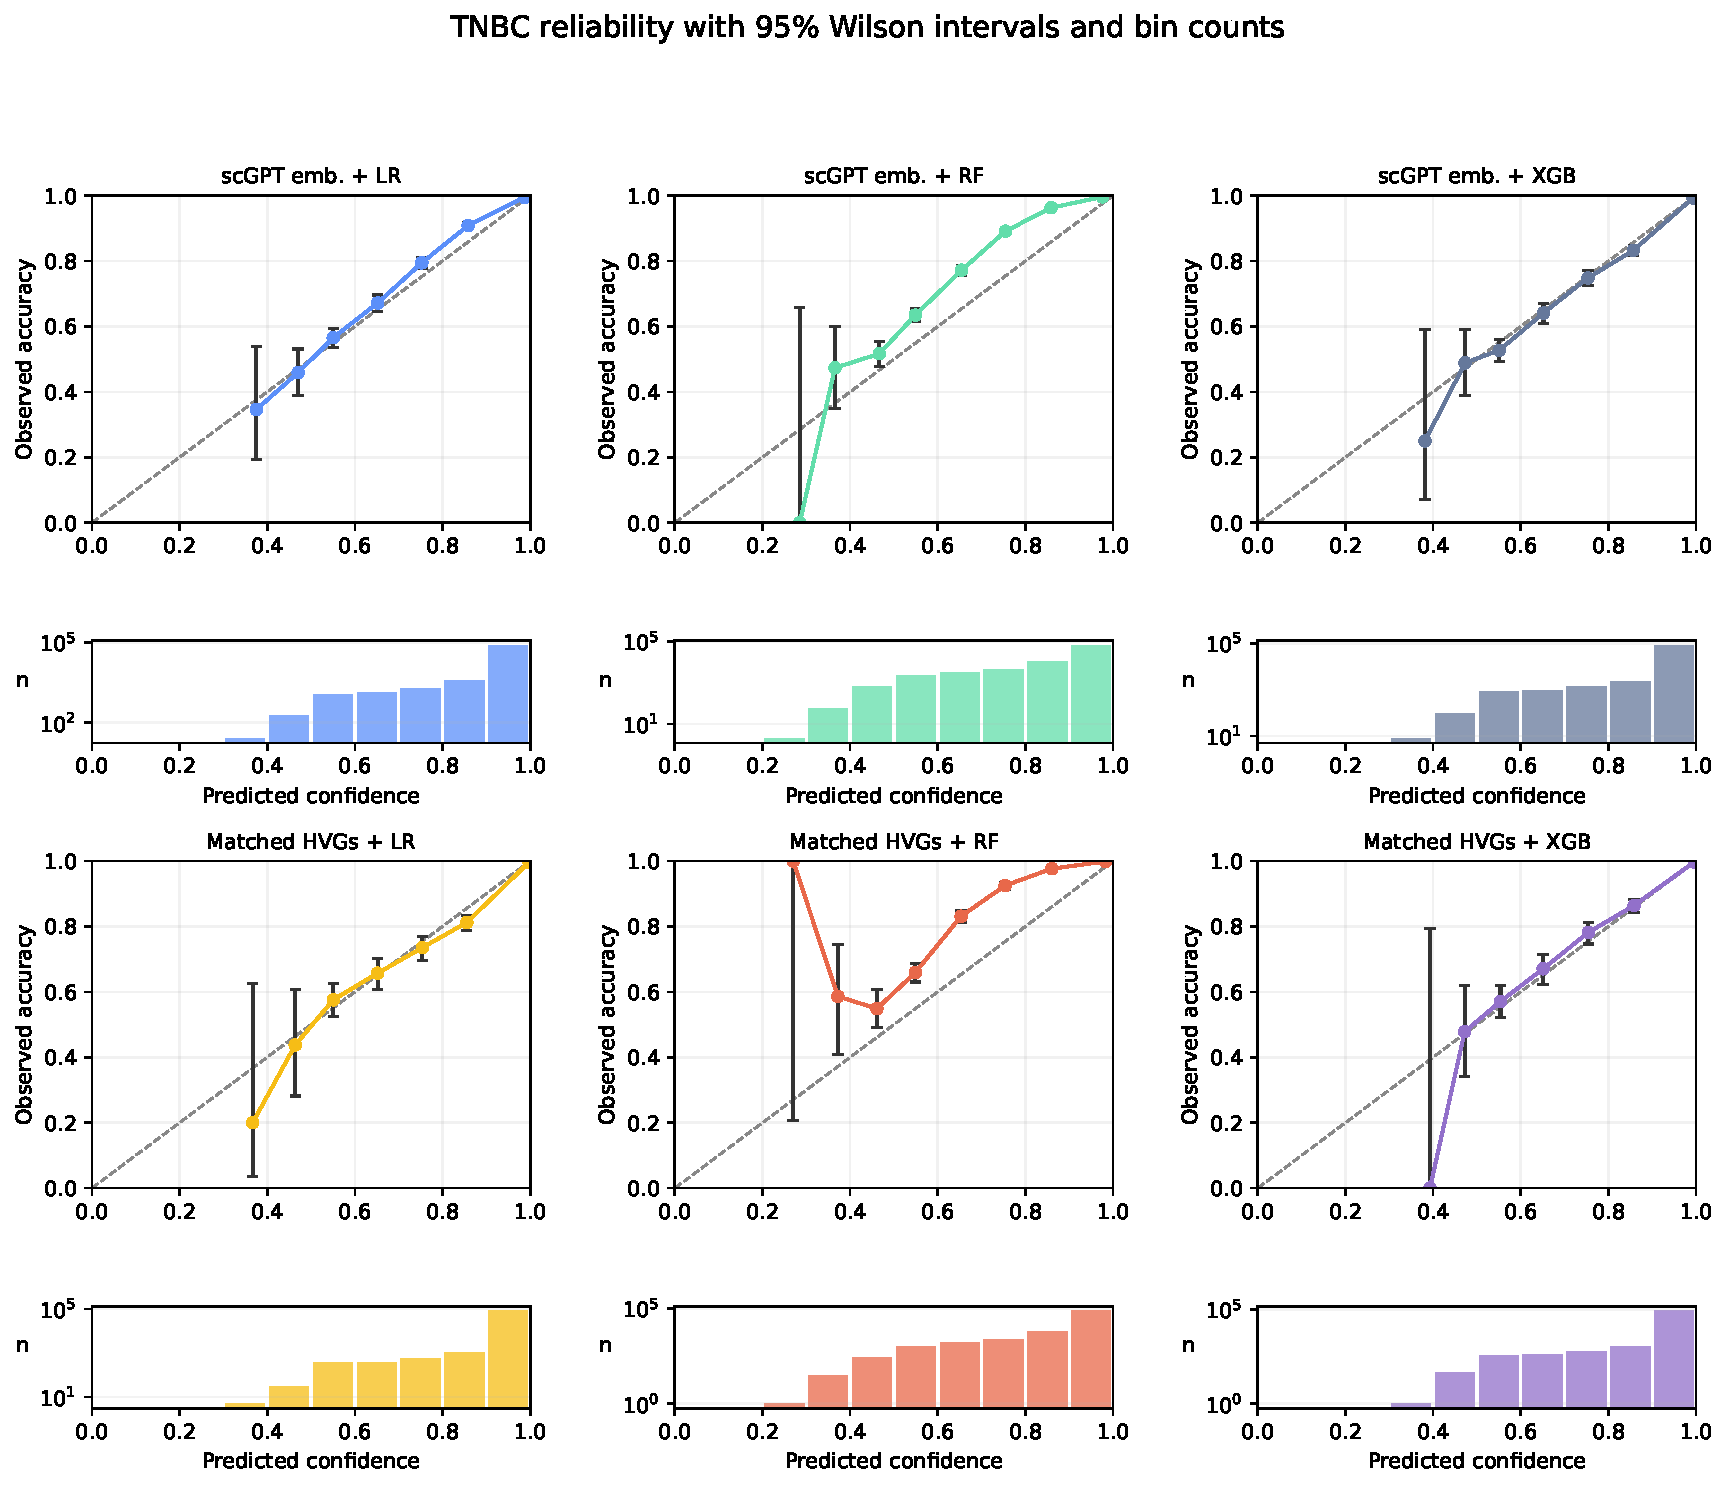
\includegraphics[width=0.98\textwidth,height=0.84\textheight,keepaspectratio]{Figure_S1_Reliability_TNBC.pdf}
\caption{Reliability of all six pipelines in the TNBC within-atlas test partition.}
\label{fig:s1}
\end{figure}

\begin{figure}[p]
\centering
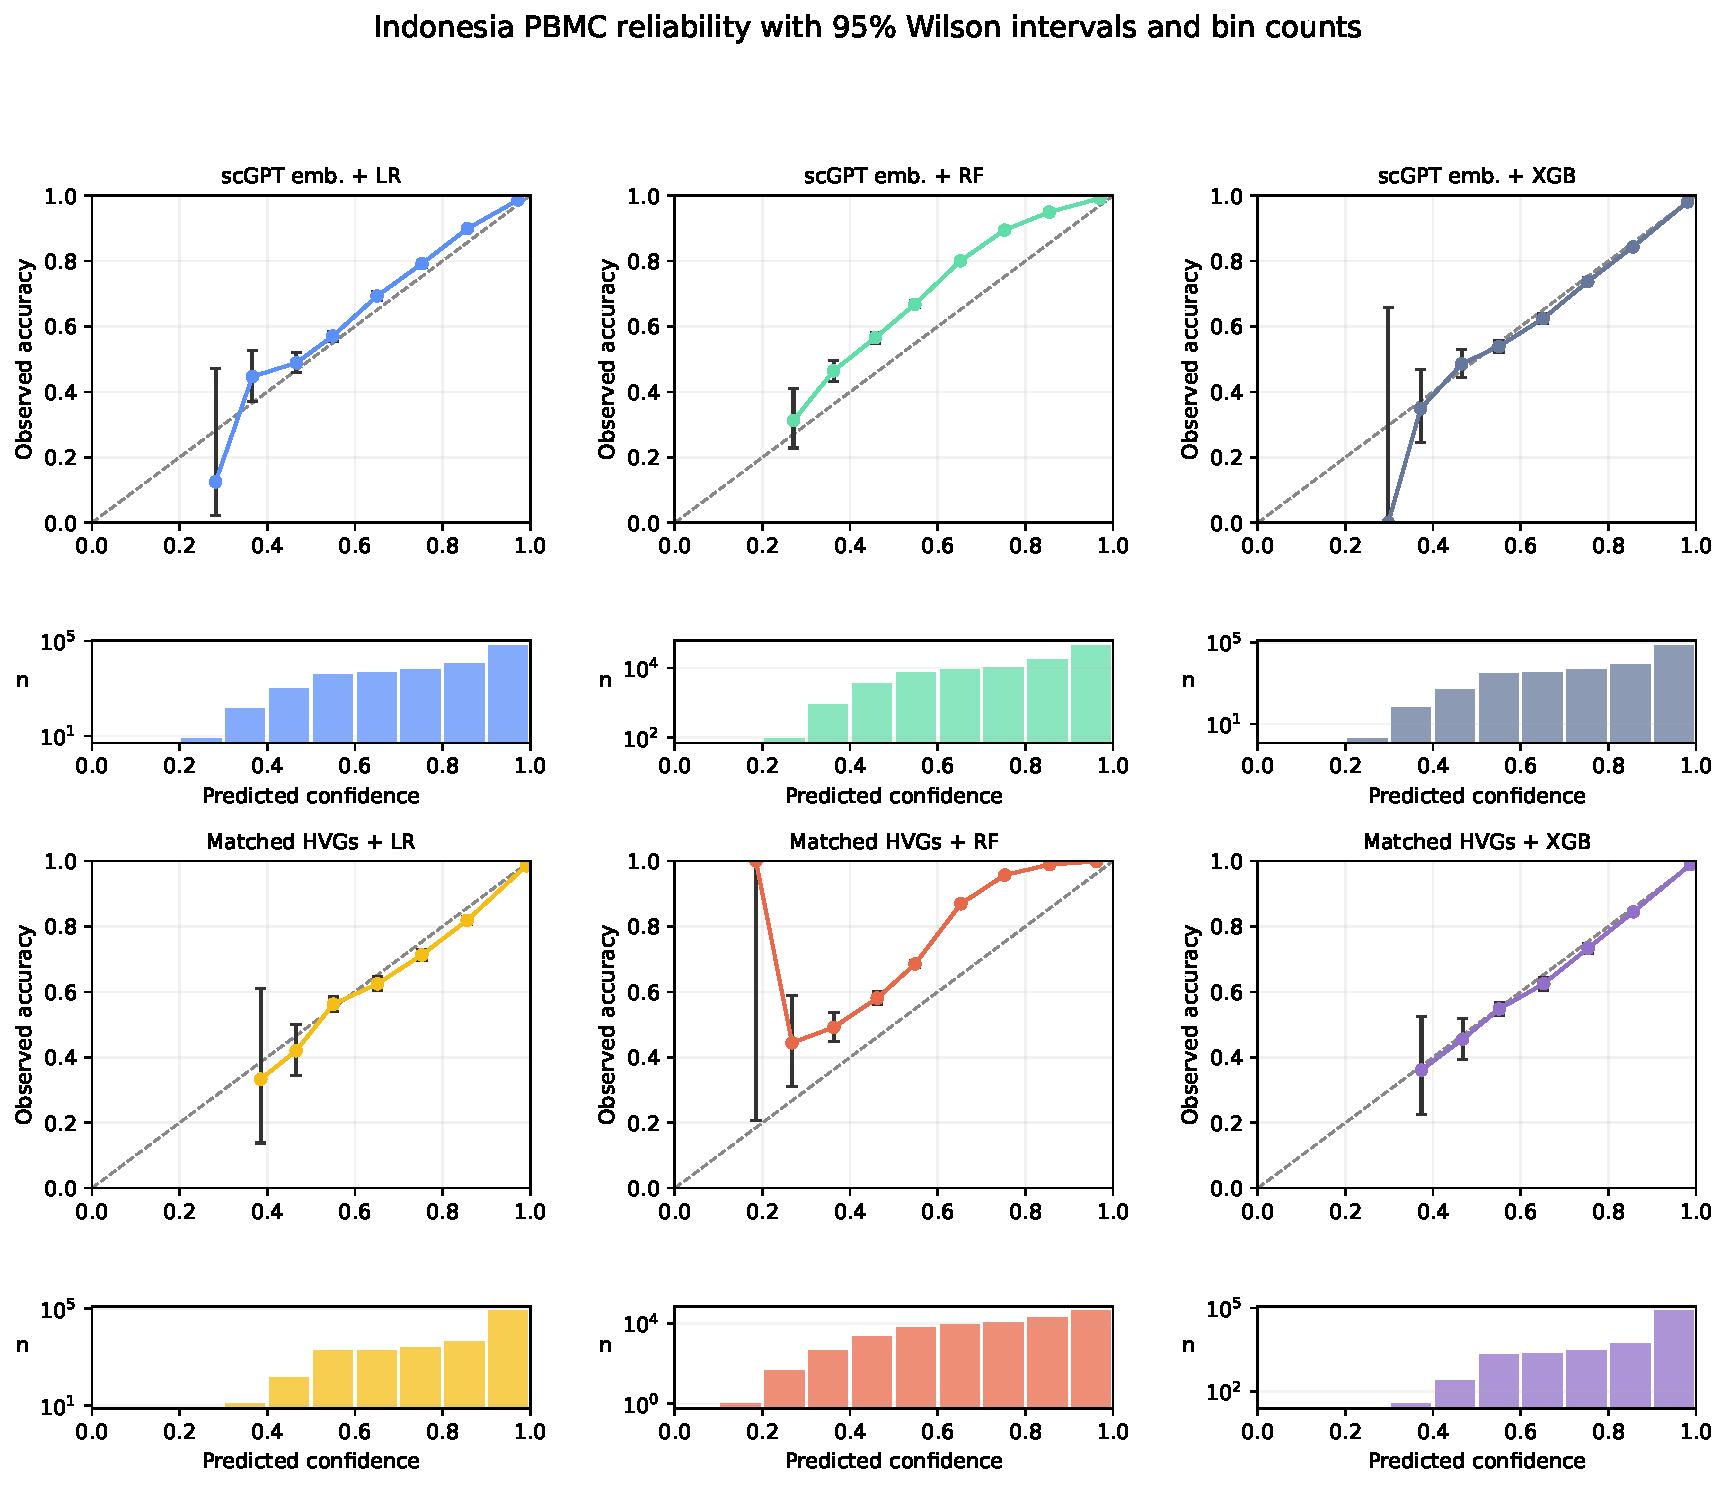
\includegraphics[width=0.98\textwidth,height=0.84\textheight,keepaspectratio]{Figure_S2_Reliability_Indonesia_PBMC.pdf}
\caption{Reliability of all six pipelines in the Indonesia PBMC within-atlas test partition.}
\label{fig:s2}
\end{figure}

\begin{figure}[p]
\centering
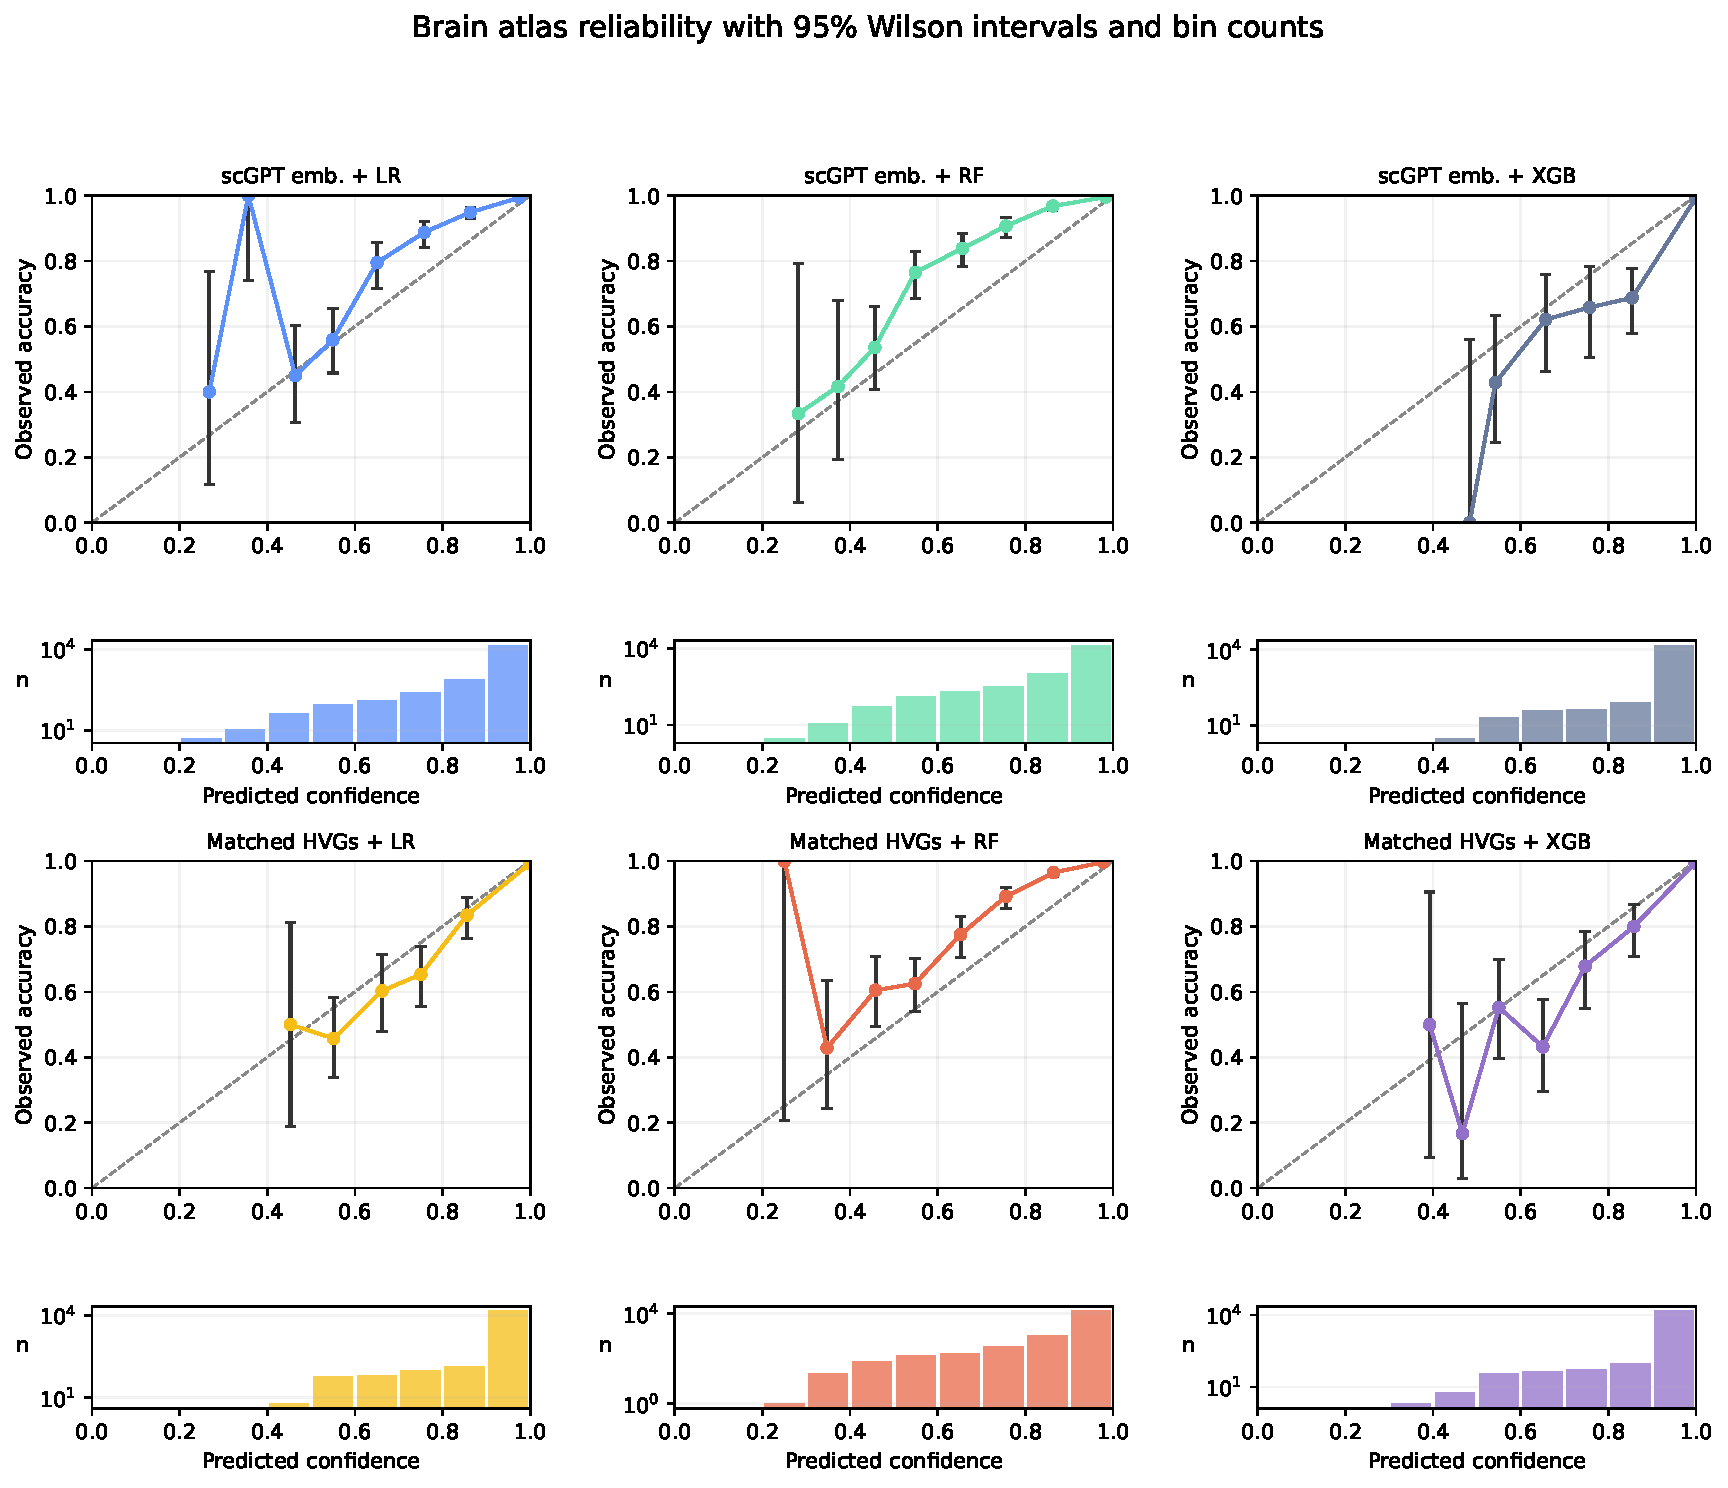
\includegraphics[width=0.98\textwidth,height=0.84\textheight,keepaspectratio]{Figure_S3_Reliability_Brain_Atlas.pdf}
\caption{Reliability of all six pipelines in the brain-atlas within-atlas test partition.}
\label{fig:s3}
\end{figure}

\begin{figure}[p]
\centering
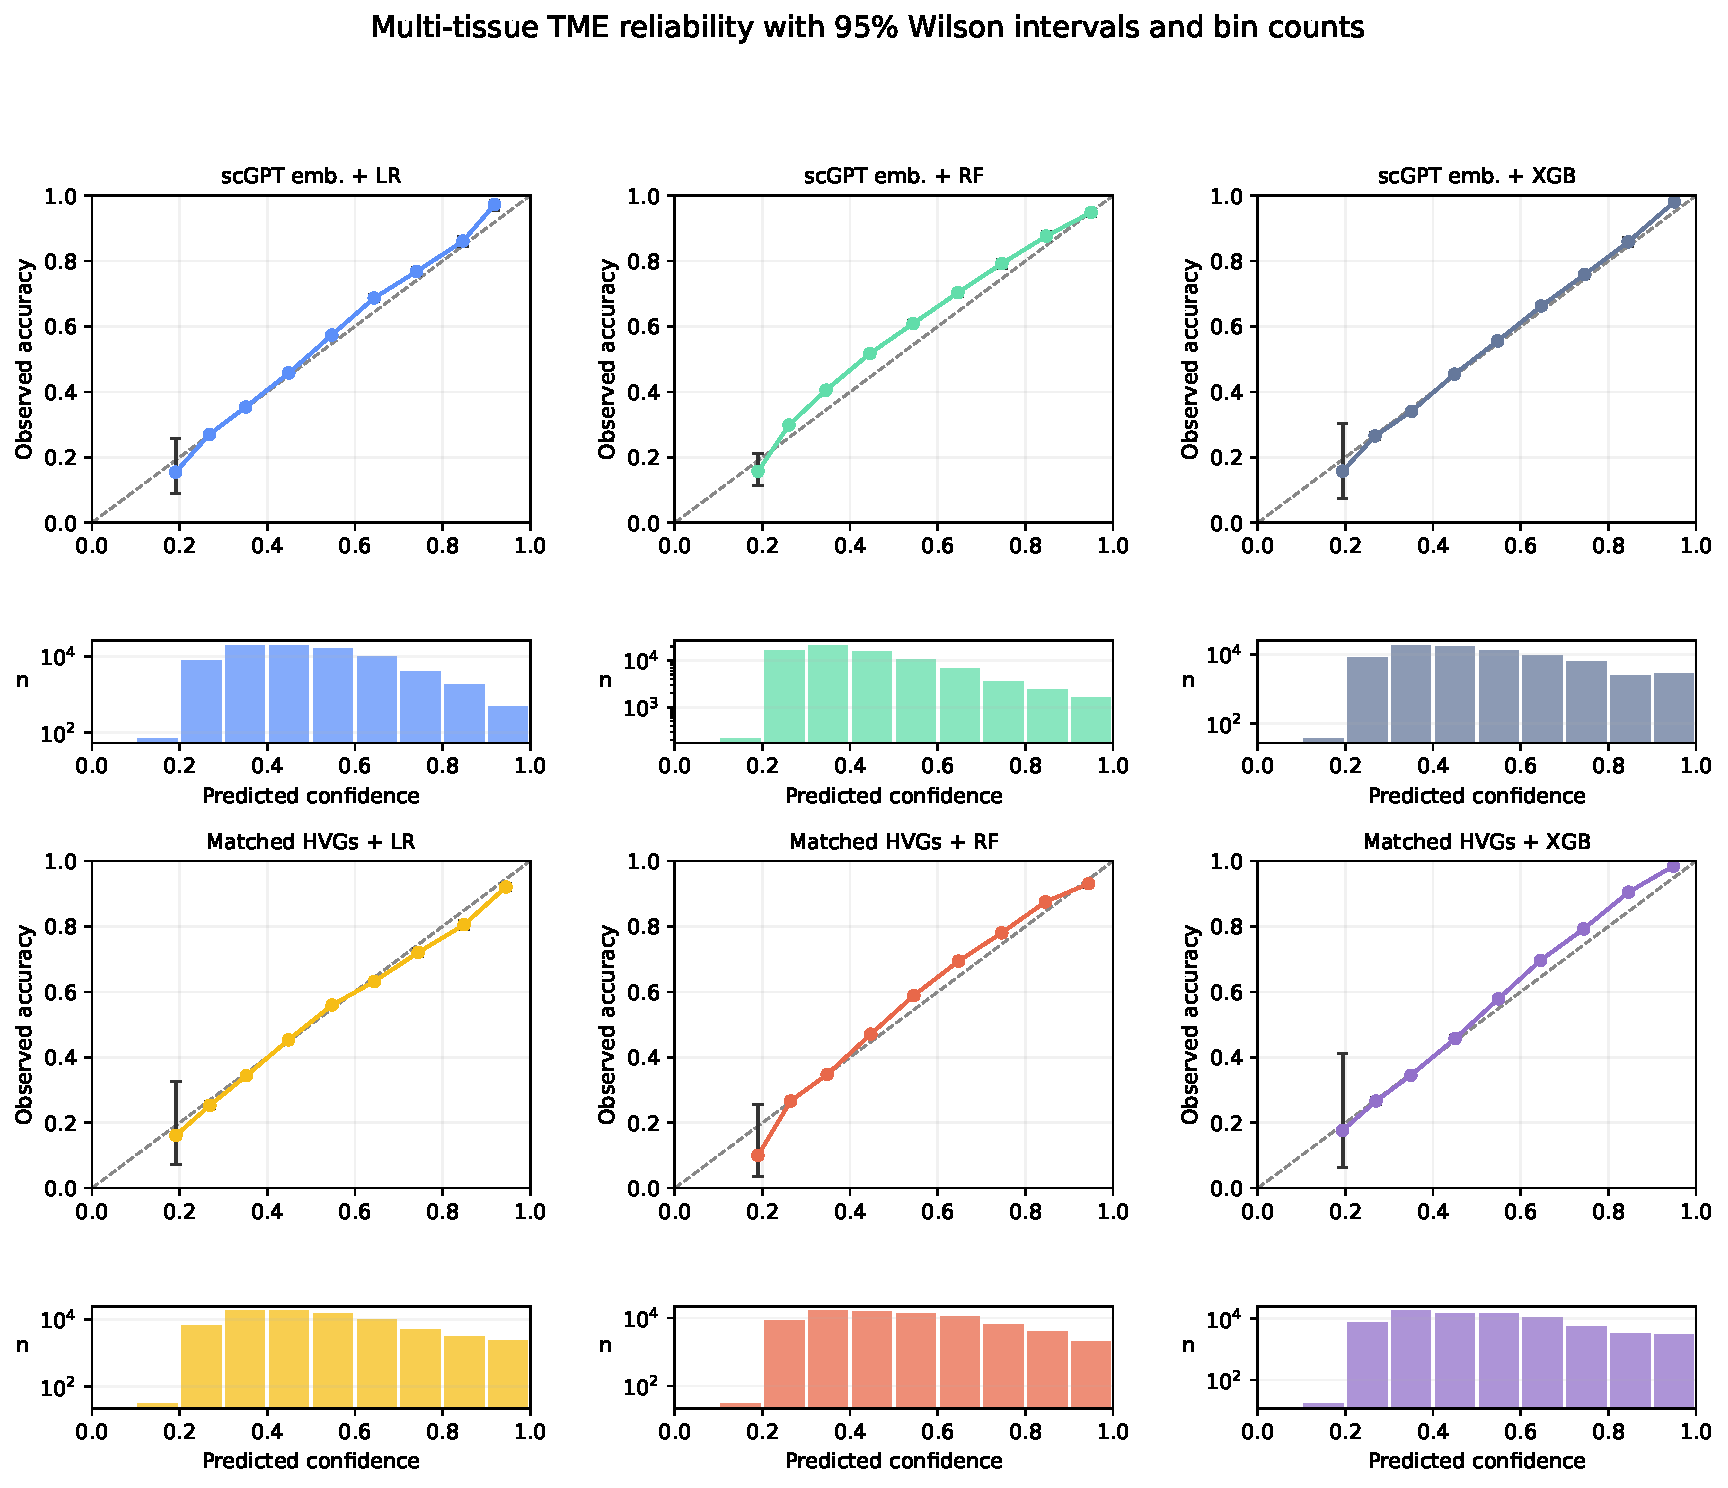
\includegraphics[width=0.98\textwidth,height=0.84\textheight,keepaspectratio]{Figure_S4_Reliability_Multi_Tissue_TME.pdf}
\caption{Reliability of all six pipelines in the multi-tissue TME within-atlas test partition.}
\label{fig:s4}
\end{figure}

\begin{figure}[p]
\centering
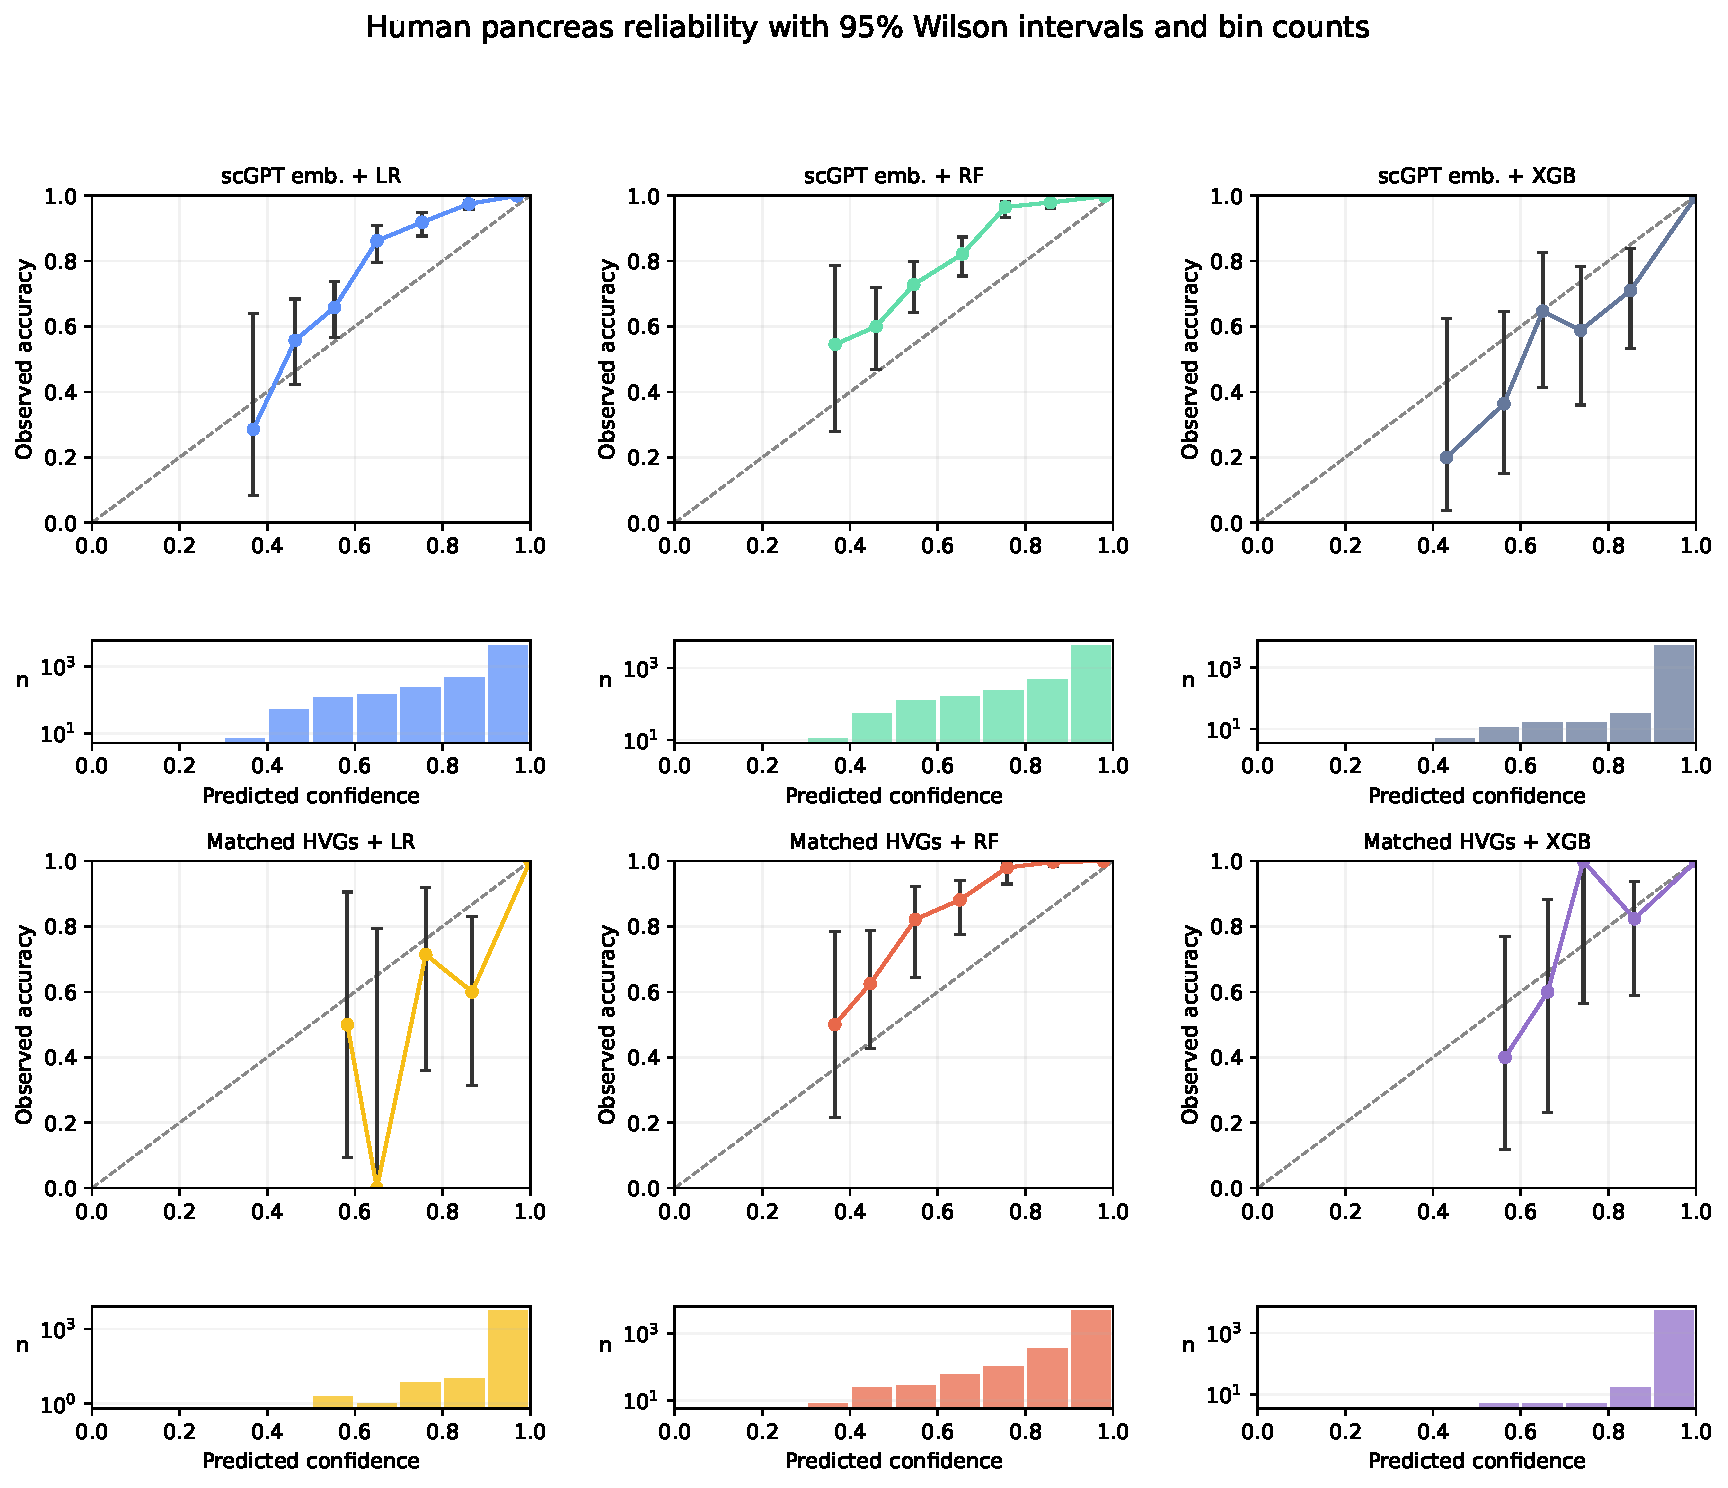
\includegraphics[width=0.98\textwidth,height=0.84\textheight,keepaspectratio]{Figure_S5_Reliability_Human_Pancreas.pdf}
\caption{Reliability of all six pipelines in the human-pancreas within-atlas test partition.}
\label{fig:s5}
\end{figure}

\begin{figure}[p]
\centering
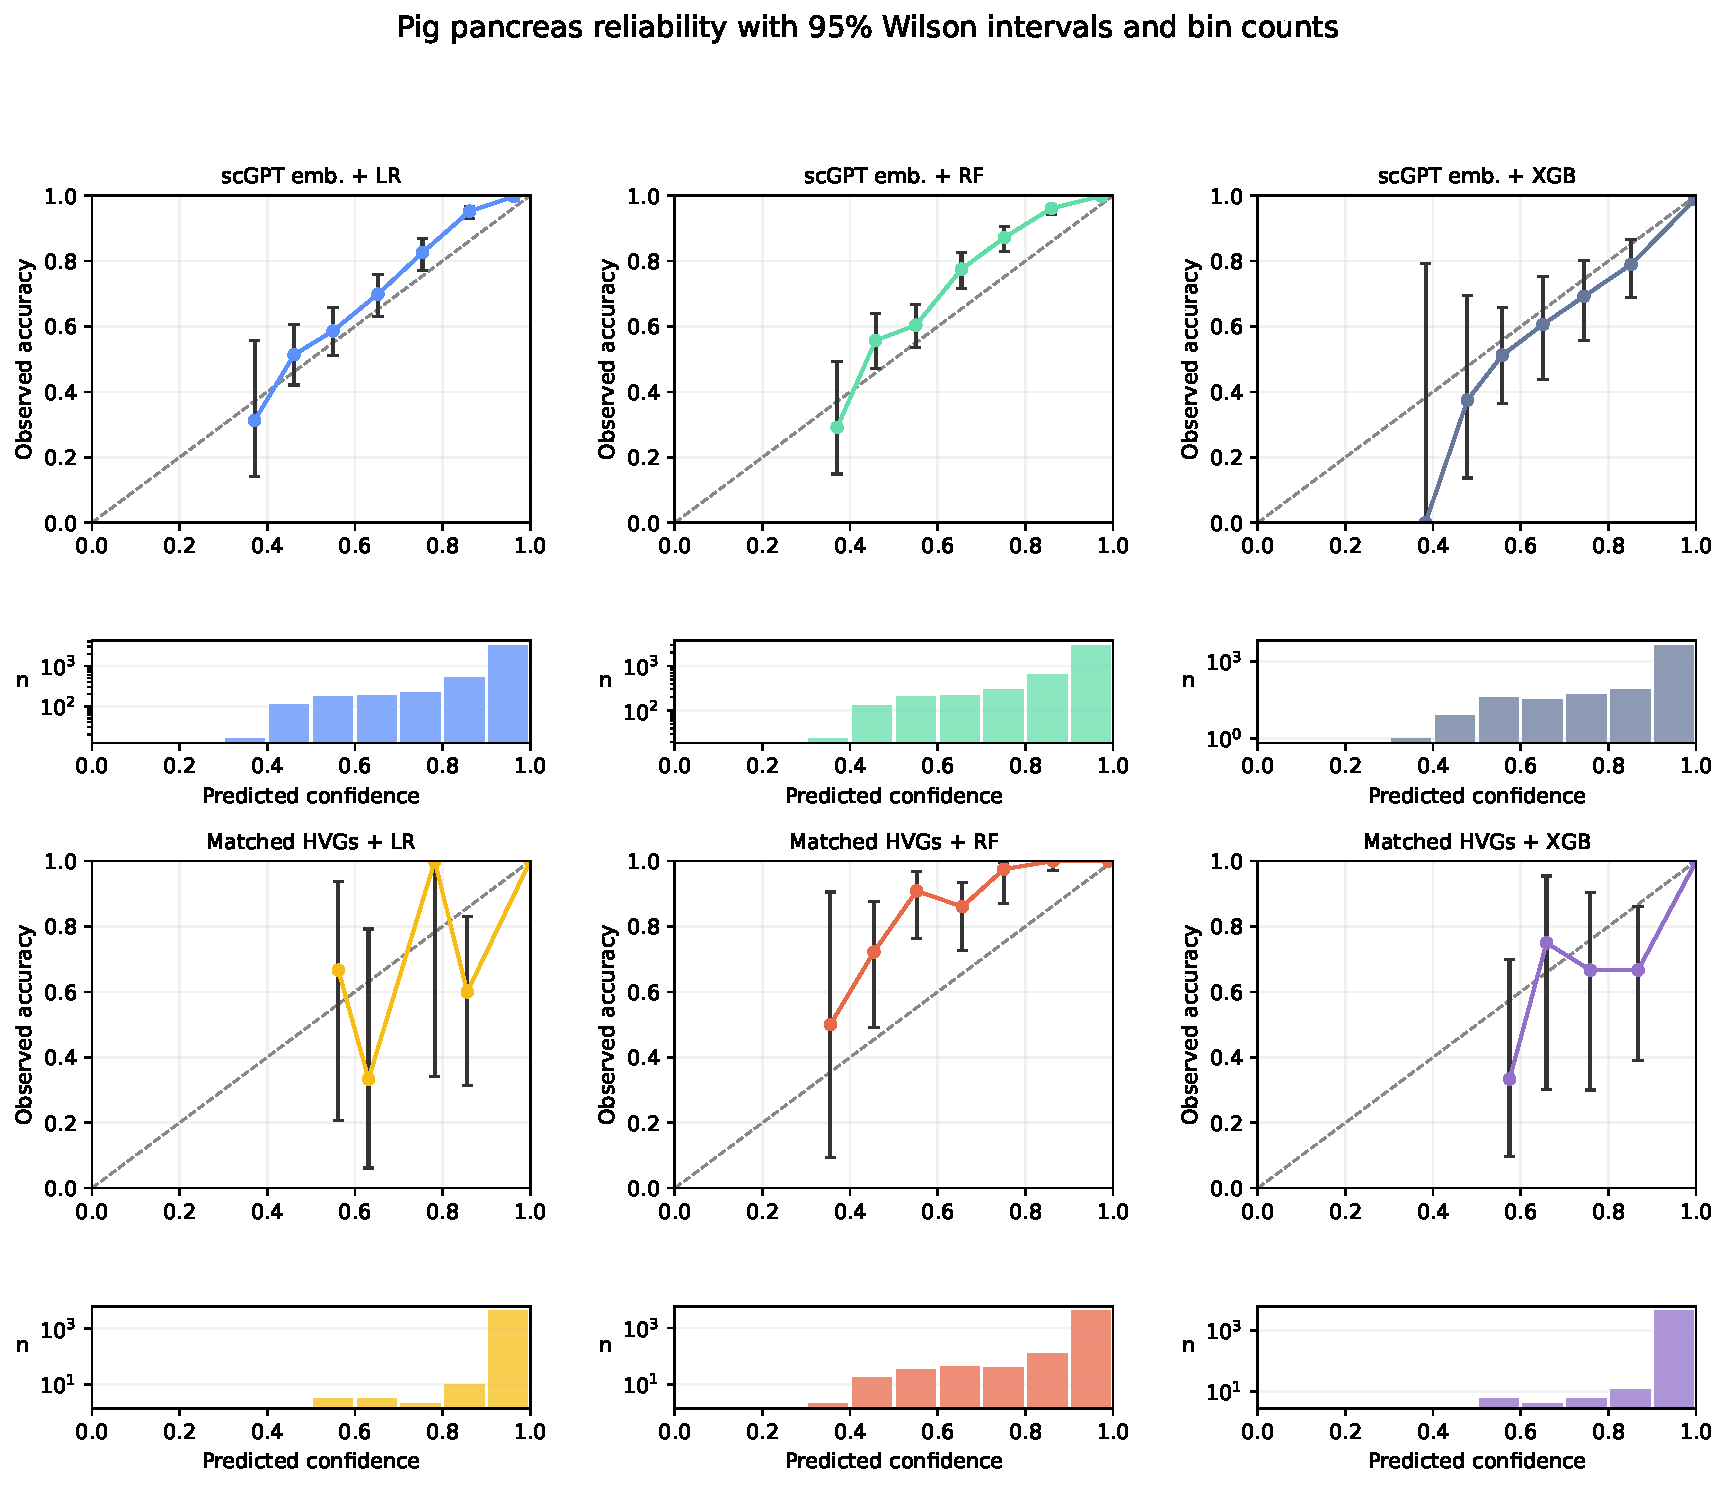
\includegraphics[width=0.98\textwidth,height=0.84\textheight,keepaspectratio]{Figure_S6_Reliability_Pig_Pancreas.pdf}
\caption{Reliability of all six pipelines in the pig-pancreas within-atlas test partition.}
\label{fig:s6}
\end{figure}

\begin{figure}[p]
\centering
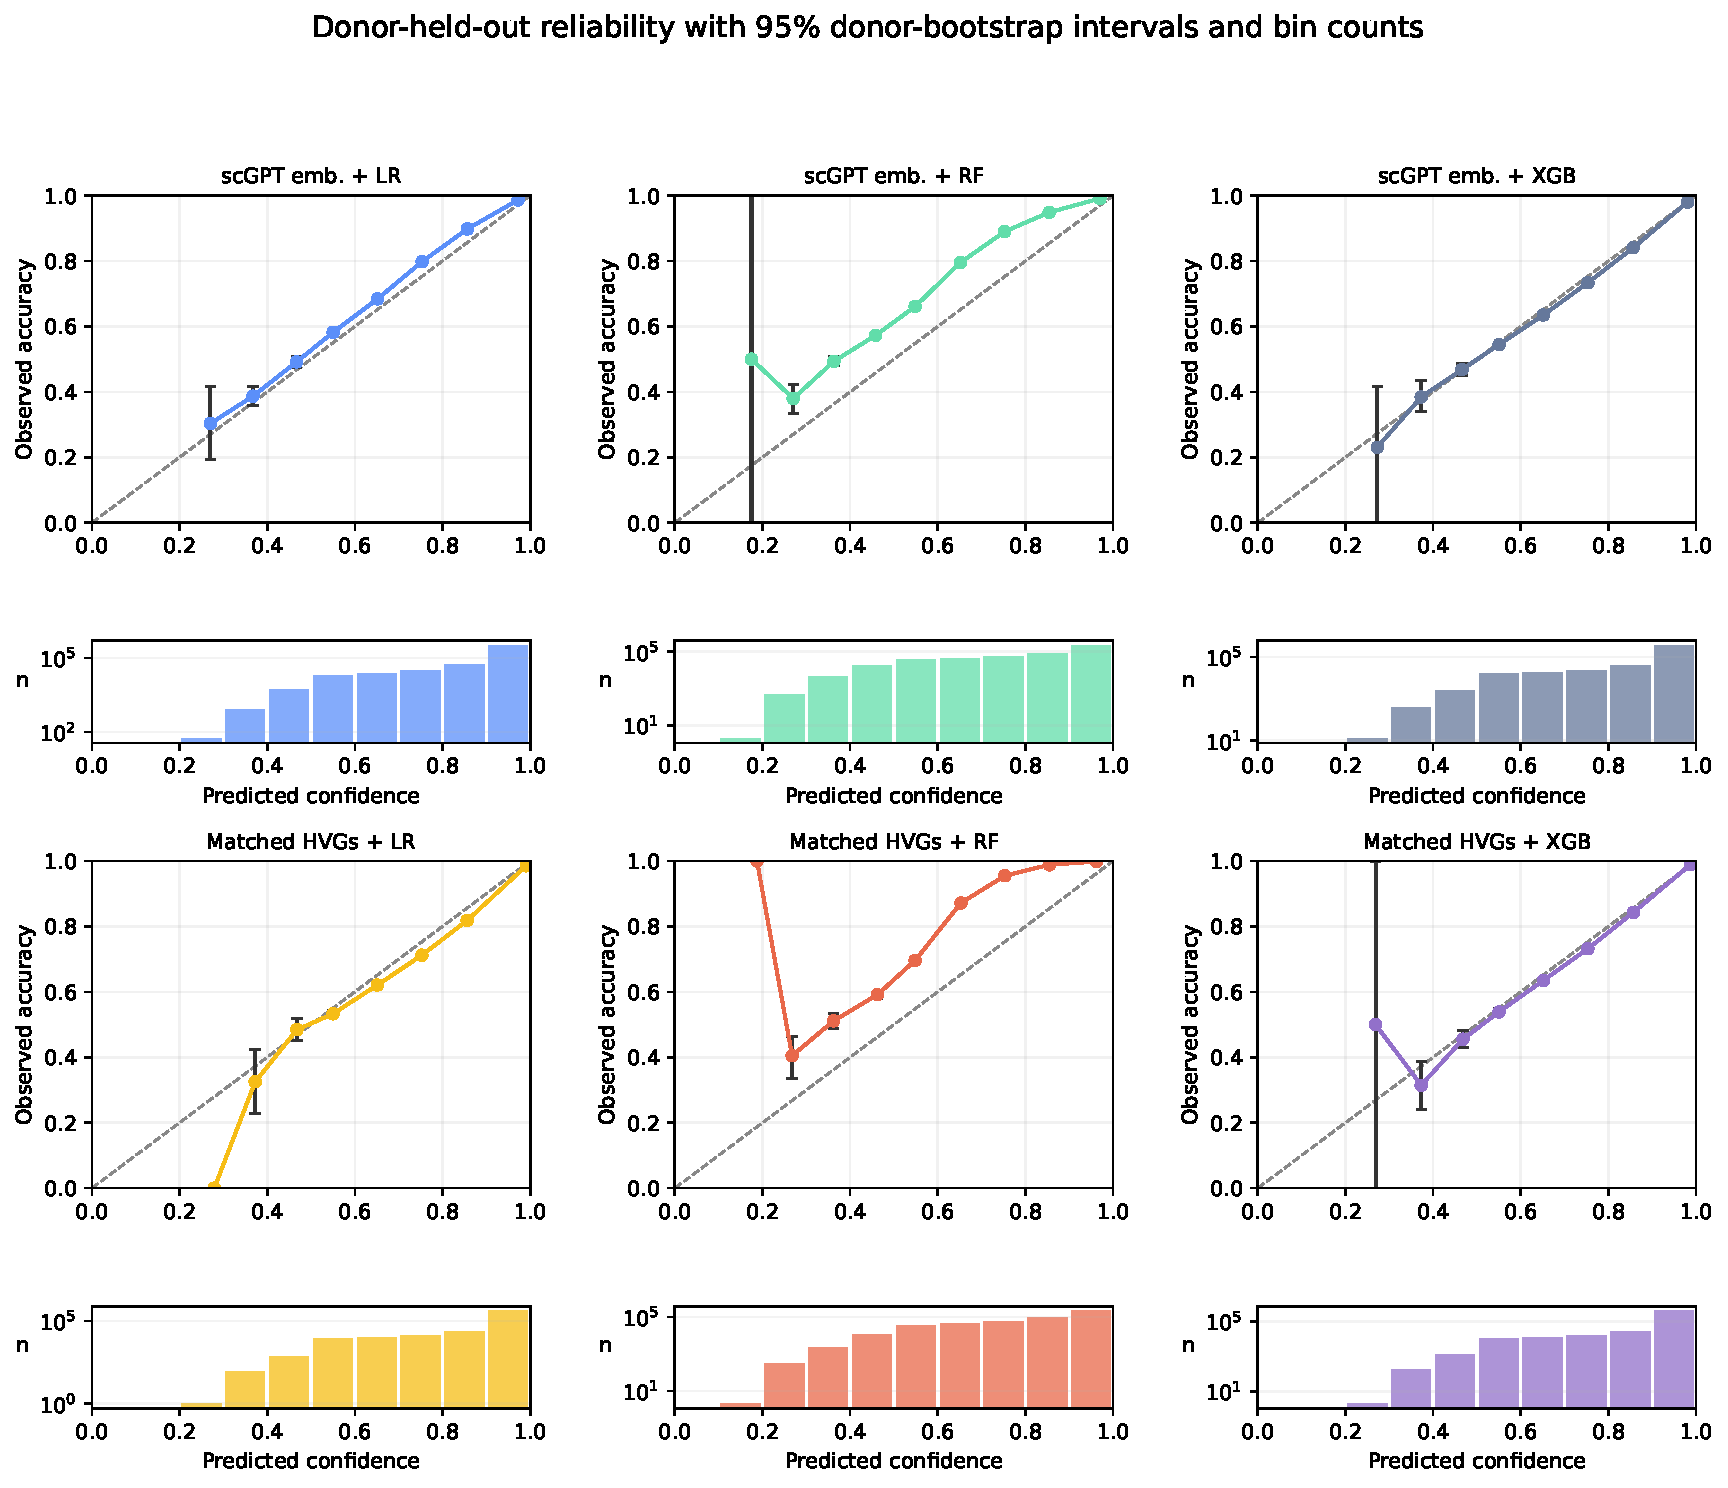
\includegraphics[width=0.98\textwidth,height=0.84\textheight,keepaspectratio]{Figure_S7_Donor_Heldout_Reliability.pdf}
\caption{Reliability of all six pipelines from pooled out-of-fold predictions on 199 Indonesia PBMC donors. Accuracy intervals resample donors and carry all cells belonging to the selected donors together.}
\label{fig:s7}
\end{figure}

\end{document}
